\documentclass{beamer}
\usetheme{Madrid}
\beamertemplatenavigationsymbolsempty
\setbeamertemplate{headline}{}
\setbeamertemplate{footline}[frame number]
\AtBeginEnvironment{frame}{\raggedright}
\usepackage{pgfplots}
\pgfplotsset{compat=1.17}
\title{Logistic Regression for Time-Window Classification}
\author{Internal Technical Note}
\date{\today}

\begin{document}

\begin{frame}{Motivation: Probabilistic Binary Decisions}
\begin{itemize}
    \item Binary label with probability \(p(y=1\mid x)\), not just a hard class.
    \item Score \(z=b+w^\top x\) is unbounded; we need a link to map it to \([0,1]\).
    \item \textbf{Score vs probability}: \(z\) only ranks samples; \(\sigma(z)\) is calibrated.
    \item Example: \(z=0.2\Rightarrow p\approx0.55\); \(z=-2\Rightarrow p\approx0.12\).
\end{itemize}
\end{frame}

\begin{frame}{Sigmoid Link and Geometry}
\begin{itemize}
    \item Sigmoid: \(\sigma(z)=\tfrac{1}{1+e^{-z}}\) squashes any score to \([0,1]\).
    \item \(z=b+w^\top x\) is the signed distance from the decision hyperplane (scaled by \(\lVert w\rVert\)).
    \item Slope is steepest at \(z=0\); samples near the boundary are most uncertain.
    \item Tiny numeric check: \(x=(1,2), w=(0.3,0.4), b=-0.5\Rightarrow z=0.6, p\approx0.65\).
\end{itemize}
\begin{center}
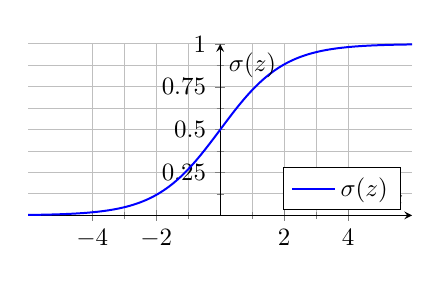
\begin{tikzpicture}[scale=0.9]
\begin{axis}[
    width=7cm, height=4cm,
    axis lines=middle,
    xlabel={$z$}, ylabel={$\sigma(z)$},
    xmin=-6, xmax=6, ymin=0, ymax=1,
    samples=200, domain=-6:6, grid=both, minor tick num=1,
    xtick={-4,-2,0,2,4}, ytick={0,0.25,0.5,0.75,1},
    legend pos=south east, legend cell align=left
]
\addplot[blue, thick] {1/(1+exp(-x))};
\legend{$\sigma(z)$}
\end{axis}
\end{tikzpicture}
\end{center}
\end{frame}

\begin{frame}{Log-Odds Are Linear}
\begin{itemize}
    \item Logit transform: \(\log \tfrac{p}{1-p} = b + w^\top x\).
    \item Log-odds affine in \(x\) \(\Rightarrow\) boundary \(w^\top x + b = 0\) is a hyperplane\\ (linear model).
    \item Monotonicity: ranking by \(z\) or by \(p\) is identical.
\end{itemize}
\end{frame}

\begin{frame}{Likelihood for Bernoulli Labels}
\begin{itemize}
    \item For i.i.d. samples, \(p_i = \sigma(b + w^\top x_i)\).
    \item Likelihood: \[\mathcal{L}(w,b)=\prod_i p_i^{y_i}(1-p_i)^{(1-y_i)}.\]
    \item Maximizing \(\mathcal{L}\) chooses \(w,b\) that make observed labels most probable.
\end{itemize}
\end{frame}

\begin{frame}{MLE and Log-Loss}
\begin{itemize}
    \item Negative log-likelihood: \[\text{NLL}=-\sum_i \big[y_i\log(p_i)+(1-y_i)\log(1-p_i)\big].\]
    \item Minimizing NLL is identical to minimizing binary cross-entropy (log-loss).
    \item Interpretation: confident wrong predictions are heavily penalized; uncertain ones less so.
\end{itemize}
\end{frame}

\begin{frame}{Regularization (L2)}
\begin{itemize}
    \item Add shrinkage: objective \(= \text{NLL} + \lambda\lVert w\rVert^2\).
    \item Geometric view: L2 keeps \(w\) inside a hypersphere; all directions penalized equally.
    \item Mitigates overfitting and stabilizes correlated features.
    \item scikit-learn: `C` is inverse strength; \(\lambda = \tfrac{1}{2C}\); smaller `C` $\Rightarrow$ stronger shrinkage.
\end{itemize}
\begin{center}
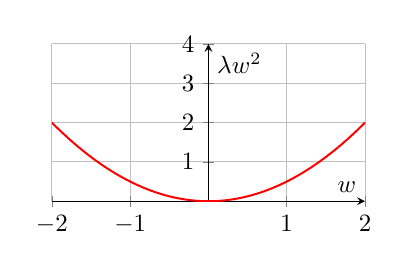
\begin{tikzpicture}[scale=0.9]
\begin{axis}[
    width=6cm, height=3.8cm,
    axis lines=middle,
    xlabel={$w$}, ylabel={$ \lambda w^2$},
    xmin=-2, xmax=2, ymin=0, ymax=4,
    samples=200, domain=-2:2, grid=major, minor tick num=0,
    xtick={-2,-1,0,1,2}, ytick={0,1,2,3,4},
]
\addplot[red, thick] {0.5*x^2};
\end{axis}
\end{tikzpicture}
\end{center}
\end{frame}

\begin{frame}{Class Imbalance}
\begin{itemize}
    \item `class\_weight="balanced"`: weight for class \(c\) is \(\tfrac{N}{2N_c}\) (inverse frequency).
    \item Loss term becomes \(\text{weight}_{y_i}\times\) log-loss, so minority-class errors count more.
    \item Helps align the effective threshold with recall/precision needs when positives are rare.
\end{itemize}
\end{frame}

\begin{frame}{Prediction, Threshold, Ranking}
\begin{itemize}
    \item `predict\_proba` returns \(p = \sigma(b + w^\top x)\); default decision uses 0.5.
    \item Lower threshold $\Rightarrow$ fewer FN but more FP; higher threshold does the opposite.
    \item ROC AUC scores the ranking by \(p\) (or \(z\)) independent of any specific threshold.
    \item Mini diagram: features \(\rightarrow z=b+w\cdot x \rightarrow \sigma(z) \rightarrow p\)\\\(\rightarrow\) threshold \(\rightarrow\) class.
\end{itemize}
\begin{center}
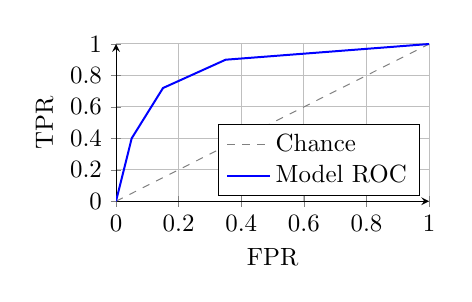
\begin{tikzpicture}[scale=0.9]
\begin{axis}[
    width=6cm, height=3.8cm,
    axis lines=left,
    xlabel={FPR}, ylabel={TPR},
    xmin=0, xmax=1, ymin=0, ymax=1,
    grid=major, legend pos=south east, legend cell align=left
]
\addplot[gray, dashed] coordinates {(0,0) (1,1)};
\addplot[blue, thick] coordinates {(0,0) (0.05,0.4) (0.15,0.72) (0.35,0.9) (1,1)};
\legend{Chance,Model ROC}
\end{axis}
\end{tikzpicture}
\end{center}
\end{frame}

\end{document}
